\section{Experiment}
\label{sec:experiments}

\subsection{Experimental setup}
\label{sec:setup}
\label{sec:cells}

\paragraph{Tasks and models.}
Our main evaluation pairs MedCalc-Bench \citep{khandekar2024medcalc} with
skills from SRA-Bench \citep{su2026srabench}, covering $55$ clinical calculators
with $20$ questions each ($1{,}100$ items). Qwen3-8B \citep{yang2025qwen3}
generates step-by-step reasoning using greedy decoding, without tools; we
evaluate its answers with the benchmark scorer. Accuracy is $74.2\%$ with the
correct skill, $34.5\%$ without a skill, and $31.5\%$ with a wrong skill.
For the decomposition and answer-format experiments, we use a synthetic
unit-conversion task with a controlled lookup table and matched wrong skills.
We also test Qwen3-0.6B, Qwen3-1.7B and Mistral-7B-Instruct-v0.3
\citep{jiang2023mistral}, and evaluate transfer to SRA-Bench's TheoremQA subset
($747$ questions and $320$ skills) using its prompt and scorer.

\paragraph{Sampling and uncertainty.}
The main MedCalc span experiments cover $467$ rescued items from $48$
calculators with at least two such items. Screening for groups whose receiver
solves no sampled item retains $135$ items from $14$ calculators. The main
depth sweep, rank curve and span-quarter comparisons use this same subset.
Appendix~\ref{app:fullscale} compares this rerun with the earlier development
samples it replaces. TheoremQA uses the same
group-based screen, which becomes an item-level screen when a skill has only
one question. We report sample sizes for each comparison. Main-text accuracy
and recovery intervals resample skill groups. Each recovery estimate uses
donor and receiver baselines on the items available for that intervention.
Incomplete reruns are excluded rather than combined into curves with changing
sample sets; complete earlier measurements are retained and identified.

\paragraph{Identity control.}
Writing the receiver's own states back should leave its output unchanged.
This identity control exposed a mismatch: capture omitted an attention mask
that decoding supplied, changing $108/1{,}766$ Qwen3-8B outcomes ($6.1\%$).
Matching the masks restores exact agreement in every corrected run, for
example on all $467$ MedCalc items and on all $9{,}308$ item--layer pairs of the
synthetic decomposition. All main-text interventions use the correction. Appendix~\ref{app:limits} records
provenance and Appendix~\ref{app:detail} implementation details. Small numerical
discrepancies can propagate through long generations \citep{he2025nondeterminism}.

\subsection{Resolving the paradox: content and answer format}
\label{sec:decomp}

\paragraph{The smaller content component carries the improvement.}
On the synthetic task with Qwen3-1.7B ($358$ items, $82$ rescued), we inject
each component of Eq.~\ref{eq:decomp} at the final prompt position. On rescued
items, the presence component recovers $0.098$ of the gain, exactly the
wrong-skill baseline; the content component recovers $0.805$, compared with
$1.000$ for full state replacement. The effect extends to failures: across
rescued, persistent-failure, kept and broken items, replacement gives
accuracies of $1.000/0.000/1.000/0.000$, while content injection gives
$0.805/0.075/1.000/0.186$. Content injection thus broadly reproduces both the
benefits and the errors induced by the skill. Recovery also depends on the
subtraction baseline. Using a skill with corrupted numbers or with shuffled sentences gives
$0.17$--$0.28$ over layers $21$--$27$, every layer measured, compared with
$0.805$ for an unrelated skill. The content component must therefore be
interpreted relative to the specified wrong skill.

\paragraph{Single-position recovery depends on answer format.}
\label{sec:onepos}
Table~\ref{tab:answerformat} compares answer formats on the synthetic task.
All three formats use the same $358$ items and all $36$ layers. For short
numeric answers, no final-position intervention recovers more than one of the
$119$ rescued items through layer $22$. The best results across layers are
$0.235$ for state replacement, $0.21$ for content and $0.008$ for presence.
These answers are one to five tokens long ($341$ of $358$ use two to four).
Patching the last $1$, $4$, $16$, $32$, $48$ and $61$ positions---$61$ is the
whole no-document prompt---recovers $0.235$, $0.261$, $0.403$, $0.403$, $0.395$
and $0.370$: the ladder saturates at $16$, and giving the patch every position
the prompt has does not raise it. For step-by-step reasoning, the skill raises accuracy from $0.000$ to
$0.989$, yet single-position replacement recovers at most one of $354$ rescued
items ($0.003$) at any layer.
These results show that the probe's success depends on answer format; they do
not establish a general limit on the information a hidden state can hold.

\begin{table}[tbp]
\caption{Final-position state replacement across answer formats, Qwen3-8B.
All formats use the same $358$ items and the same skill, with every layer
($0$--$35$) tested. Recovery is the best state-replacement result over layers
on each format's rescued items. The identity intervention reproduces the
unpatched output on every item and layer.}
\label{tab:answerformat}
\centering\small
\begin{tabular}{@{}lrrrr@{}}
\toprule
Answer format & Tokens & Evaluated & Rescued & Best recovery \\
\midrule
Multiple choice & 1 & 358 & 94 & $1.000$ \\
Numeric answer & 1--5 & 358 & 119 & $0.235$ \\
Chain of thought & Hundreds & 358 & 354 & $0.003$ \\
\bottomrule
\end{tabular}

\end{table}

The corrected clinical comparison tests the final position and larger sets
of positions after the skill at layer $8$, using the same $135$ items and
wrong-skill receiver as span injection (Figure~\ref{fig:channels}). The last
$1$, $16$ and up to $256$ positions recover $0.03$, $0.06$ and $0.05$,
respectively. Earlier multi-layer probes
are reported separately in \extref{Appendix}{app:onepos}{the extended version}; the complete matched
comparison here concerns layer $8$.

\subsection{The skill span supports content injection}
\label{sec:battery}

\paragraph{Changing the intervention positions restores recovery.}
We next apply Eq.~\ref{eq:inject} across the skill's own positions. At layer
$8$, span injection raises accuracy from $0.000$ to $0.815$ on the screened
$135$-item subset, recovering $0.89$ of the donor's gain
(Table~\ref{tab:big40}). Figure~\ref{fig:channels} compares this with writing
donor states at the final position, the final $16$ positions, or up to $256$
positions after the skill, using the same layer, items and receiver.
All positions outside the chosen intervention retain their receiver states.

\begin{figure*}[tbp]
\centering
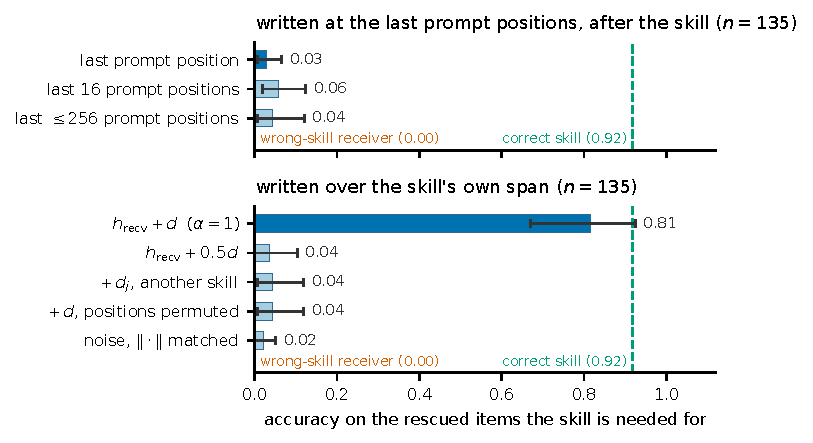
\includegraphics[width=\textwidth]{fig-channels-medcalc.pdf}
\caption{Matched position comparison on MedCalc with Qwen3-8B after the fix.
Both panels use layer $8$, the same wrong-skill receiver and $135$ items from
$14$ calculators. Left: donor states written at the last $1$, $16$, or up to
$256$ available positions after the skill. Right: interventions over the skill
span. The dashed line marks correct-skill accuracy; the dotted line marks
receiver accuracy. Error bars are calculator-bootstrap $95\%$ intervals.}
\label{fig:channels}
\end{figure*}

\paragraph{Dose, transfer, order and noise controls.}
Recovery changes nonlinearly with injection strength. On the screened subset
($n=135$, $14$ calculators), $\alpha=0.4,0.5,0.55$ gives
$0.04,0.04,0.14$ recovery, while $0.6,0.7,1.0$ gives $0.53,0.87,0.89$;
doubling the injection to $\alpha=2$ reduces recovery to $0.77$. Most of the
increase occurs between $0.55$ and $0.7$. To test content specificity, we
compare correct and other-skill injections over a common prefix length: the
correct prefix recovers $0.65$, whereas content from an unrelated skill
recovers $0.05$. A same-family mean control recovers $0.12$ on its $41$ eligible items.
Permuting positions also gives $0.05$, norm-matched Gaussian noise
gives $0.02$, and the identity control gives $0.00$. These controls show that
recovery depends on the injected content and its arrangement across positions,
rather than perturbation size alone.

\begin{table*}[tbp]
\caption{Span interventions on the screened MedCalc subset: $135$ items from
$14$ calculators, selected from $467$ rescued items across $48$ calculators
by requiring the wrong-skill receiver to solve no sampled item in a group.
The same-family control is available on $41$ items. Each row uses baselines
matched to its own items in Eq.~\ref{eq:rho}; accuracy intervals resample
calculators. Table~\ref{tab:replication} gives the interval for full-span recovery.}
\label{tab:big40}
\centering
\small
\begin{tabular}{@{}lrccc@{}}
\toprule
intervention & $n$ & accuracy & CI$_{95}$ & recovery $\rho$ \\
\midrule
\emph{correct skill in context} & $135$ & $0.919$ & $[0.844,\,0.976]$ & $+1.00$ \\
$h_{\text{recv}}+\dvec$ \ (full span) & $135$ & $0.815$ & $[0.670,\,0.925]$ & $+0.89$ \\
correct content, shared prefix & $135$ & $0.593$ & $[0.336,\,0.820]$ & $+0.65$ \\
half dose ($\alpha=0.5$) & $135$ & $0.037$ & $[0.000,\,0.103]$ & $+0.04$ \\
another skill (individual donor) & $135$ & $0.044$ & $[0.007,\,0.119]$ & $+0.05$ \\
mean from another skill family & $135$ & $0.044$ & $[0.012,\,0.102]$ & $+0.05$ \\
mean from the same skill family & $41$ & $0.122$ & $[0.000,\,0.250]$ & $+0.12$ \\
positions permuted & $135$ & $0.044$ & $[0.007,\,0.118]$ & $+0.05$ \\
norm-matched Gaussian noise & $135$ & $0.022$ & $[0.000,\,0.051]$ & $+0.02$ \\
\emph{identity intervention} & $135$ & $0.000$ & $[0.000,\,0.000]$ & $+0.00$ \\
\emph{wrong skill, unpatched} & $135$ & $0.000$ & $[0.000,\,0.000]$ & $+0.00$ \\
\bottomrule
\end{tabular}

\end{table*}

The receiver screen affects how these controls should be interpreted. On the
$34$ excluded calculators, the wrong-skill receiver already solves some items.
Other-skill content recovers $0.17$ on these groups ($n=332$), compared with
$0.05$ on the retained groups ($n=135$); noise recovers $0.10$ versus $0.02$.
This pattern is consistent with perturbations enabling knowledge already
available to the model, although it does not establish that mechanism.
A separate caveat is intervention size: skill spans in the screened subset
contain $365$--$1{,}630$ positions, far more than a single-position probe;
\S\ref{sec:posbudget} separates the number of written positions from their
arrangement.

\subsection{Which positions carry the effect}
\label{sec:posbudget}

Span injection writes $365$--$1{,}630$ positions; the final-position probe
writes one. To separate the arrangement of the span from the amount of state
it injects, we fix the number of written positions $B$ and vary only which
positions receive their own donor states, on the same $135$ items, layer and
receiver as Table~\ref{tab:big40} (Figure~\ref{fig:posbudget}).
\emph{Quantity does not explain recovery.} Evenly spaced or random subsets
recover at most $0.15$, even at half the span and half its content energy;
choosing the positions with the largest content change recovers at most
$0.12$; and writing states after the span stays at or below $0.07$, whether
the last $1$ to $234$ prompt positions at layer $8$ or the last $1$, the last
$16$ or all of them at each of seven layers from $4$ to $30$.
\emph{Contiguity does.} The same $256$ positions written as one block recover
$0.37$, and cutting that block into $2$, $4$, $8$, $16$ and $32$ evenly spaced
pieces lowers recovery to $0.24$, $0.22$, $0.13$, $0.08$ and $0.08$ at constant
budget and energy (one versus $32$ pieces: $+0.29$ [$0.09,0.48$], McNemar
$p<10^{-6}$). \emph{Location matters within the span.} A half-span block
centred on the procedure section recovers $0.82$ [$0.67,0.93$], close to the
full span; centred on the worked example it recovers $0.18$. \emph{Placement
must be exact.} Shifting every state by one position recovers $0.15$--$0.22$
with or without wrap-around, whereas leaving out the first or last $16$
positions and writing the rest in place keeps $0.89$--$0.92$. The skill's
effect is therefore carried by contiguous, correctly placed states of its
procedure-bearing tokens, not by the number of positions written or the
energy injected.

\begin{figure*}[tbp]
\centering
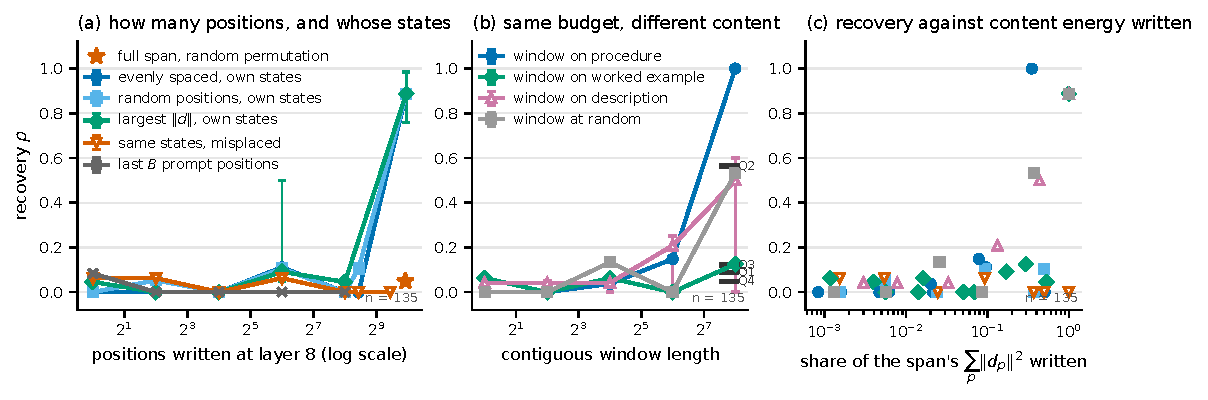
\includegraphics[width=0.72\textwidth]{fig-posbudget.pdf}
\caption{Position budget on MedCalc with Qwen3-8B, layer $8$: the same $135$
screened items ($14$ calculators) and wrong-skill receiver in every panel;
the dashed line is the whole span written in place ($\rho=0.89$). (a) $B$
positions, each written with its own donor state (evenly spaced, random, or
largest $\|d_p\|$), the same states written half a span away, or the last
$B$ prompt positions after the span. (b) A fixed budget written as $N$
contiguous blocks; dotted lines are random single positions at the same
budget. (c) One contiguous block centred on a section of the skill. (d) The
whole span displaced by $D$ positions, cyclically or without wrap-around;
triangles write it in place without its first or last $1$ or $16$
positions. Error bars are calculator-bootstrap $95\%$ intervals.}
\label{fig:posbudget}
\end{figure*}

\subsection{Skill identity and content within the span}
\label{sec:whose}

Table~\ref{tab:skillcontent} examines which content supports transfer and
whether it depends on the question. Of four contiguous span quarters, the
formula quarter gives the largest standalone recovery ($0.56$), compared with
$0.89$ for the full span. With the skill before the question, causal masking
prevents its states from depending on later question tokens: states are
identical across instances at equal prompt length and nearly identical
otherwise (cosine $\ge0.994$ over all $48$ calculators). Placing the skill after the question allows
such dependence. Even then, states from other instances of the same skill
recover $0.98$ at layer $8$, close to the current instance's $1.02$. At layer
$16$, the gap widens to $0.29$ versus $0.49$, while the instance-specific
remainder recovers little on its own. Early transfer therefore relies largely
on content shared across questions, with greater question dependence later.

\begin{table}[tbp]
\caption{Content and question dependence of span states, Qwen3-8B after the fix.
Top: each contiguous quarter is injected separately, on $135$ items from $14$
calculators. Bottom: with the skill after the question, content shared across
other instances and the instance-specific remainder are injected separately,
on $151$ items from $17$ calculators. Each comparison uses its screened subset
from the larger rerun. All entries report recovery $\rho$.}
\label{tab:skillcontent}
\centering\small
\begin{tabular}{@{}lcc@{}}
\toprule
\multicolumn{3}{@{}l}{\textit{Skill quarters, layer 8, skill before question} ($n=135$)} \\
Injected content & \multicolumn{2}{c}{Recovery $\rho$} \\
\midrule
Prose description & \multicolumn{2}{c}{$0.09$} \\
Formulas & \multicolumn{2}{c}{$0.56$} \\
Tool signatures & \multicolumn{2}{c}{$0.12$} \\
Worked example & \multicolumn{2}{c}{$0.05$} \\
Full span & \multicolumn{2}{c}{$0.89$} \\
\midrule
\multicolumn{3}{@{}l}{\textit{Question dependence, skill after question} ($n=151$)} \\
Injected content & Layer 8 & Layer 16 \\
\midrule
This instance & $1.02$ & $0.49$ \\
Other instances of the same skill & $0.98$ & $0.29$ \\
Instance-specific remainder & $0.03$ & $0.05$ \\
\bottomrule
\end{tabular}

\end{table}

Two completed corrected controls test whether a shared shift or a change in
state norm could explain recovery. Averaging content differences across skills
recovers only $0.03$ with the skill first ($n=135$) and $0.04$ with it last
($n=151$). Rescaling patched states to match the receiver's norm at each
position preserves $0.87$ recovery, compared with $0.89$ without rescaling.
In the corrected rerun, layer-$16$
recovery is $0.49$ with the skill last ($151$ items, $17$ calculators) and
$0.06$ with it first ($135$ items, $14$ calculators). Because these screens
retain different subsets, the contrast suggests sensitivity to prompt order
but is not a matched estimate of its effect (\extref{Appendix}{app:belongs}{extended version}).

\subsection{Rank required to recover the skill's effect}
\label{sec:rank}

We next inject the truncated matrix in Eq.~\ref{eq:rank} to measure how
recovery depends on the retained directions. Each intervention preserves the
same skill-specific mean at every span position, so the comparison tests how
much variation across positions is needed beyond that mean. At layer $8$ on
the screened MedCalc subset ($135$ items, $14$ calculators), recovery is
$0.07,0.05,0.12$ for $k=4,16,32$, rising to $0.63$ at $64$ and $0.77$ at
$128$, and reaching the untruncated $0.89$ at $256$ (Figure~\ref{fig:rank}).
Keeping the bottom $4$ to $128$ directions recovers at most $0.04$.
Recovery therefore depends on which directions are retained: the leading
directions support most of the measured effect, but a small number is
insufficient under this intervention.

For comparison across models, we summarise each curve by $k^{*}$: the first
rank reaching halfway from recovery at $k=16$ to the maximum on the fixed grid
$\{16,32,64,128\}$, with interpolation in $\log_2 k$. We call this the
\emph{rank knee}; it is not the minimum rank needed for full recovery.
Qwen3-8B gives $k^{*}=47$ [$43,55$], approximately $1.1\%$ of its hidden
width. \extref{Appendix}{app:rank2}{The extended version} reports development and deeper-layer curves.
These measurements describe what the injected representation can recover,
rather than directly measuring the model's unmodified computation: truncated
states may activate pathways absent from an unpatched run
\citep{makelov2024illusion}.

\begin{figure*}[tbp]
\centering
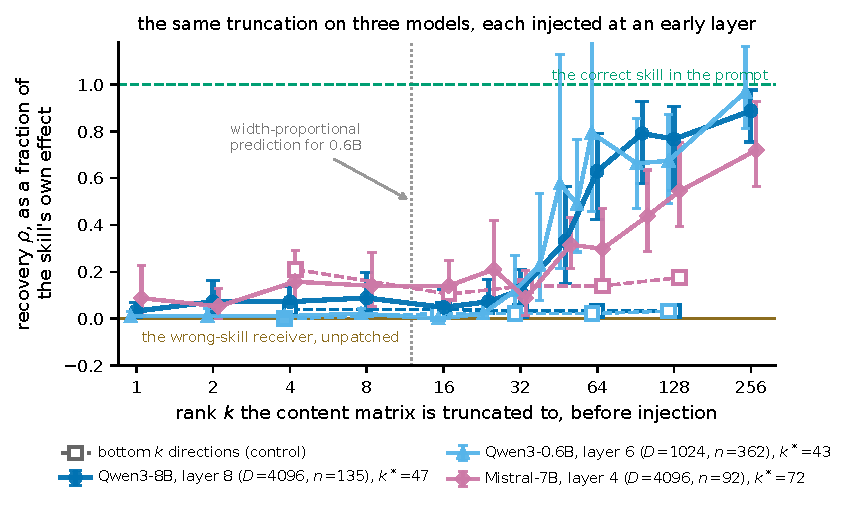
\includegraphics[width=0.88\textwidth]{fig-rank-medcalc.pdf}
\caption{Recovery after retaining $k$ leading centred directions and restoring
the positional mean, on MedCalc after the fix. Each model is injected at an
early layer. Despite a fourfold difference in hidden width, Qwen3-0.6B and
Qwen3-8B have similar rank knees ($43$ and $47$); Mistral-7B, with the same
width as Qwen3-8B, has $k^{*}=72$ [$46,94$]. Untruncated recovery is $0.89$,
$0.91$ and $0.84$, respectively, on each model's screened subset ($135$, $362$
and $92$ items). Both Qwen models reach that value by $k=256$ and Mistral-7B
at $k=384$. Dashed curves retain bottom directions. Error bars are
calculator-bootstrap $95\%$ intervals. Only complete rank experiments are
plotted.}
\label{fig:rank}
\end{figure*}

\subsection{Transfer depth and continued use of the skill}
\label{sec:where}
\label{sec:depth}

\paragraph{Span replacement and attention knockout separate in depth.}
Figure~\ref{fig:transferreading} compares transfer through span replacement
with continued use through attention on Qwen3-8B. Every layer is measured,
and both interventions are read on the same screened items. Replacement
recovers $0.92$--$0.98$ through layer $7$, $0.89$ at $8$ and $0.74$ at $12$
of $36$, then $0.16$ at $13$ and at most $0.07$ from $14$ onward ($n=135$,
$14$ calculators); the drop between layers $12$ and $13$ accounts for most of
the decline. We define the crossing below $\rho=0.5$ as the \emph{transfer
boundary} (labelled ``handover'' in the figures and tables). The
log-probability of the donor's generated reasoning also drops between these
layers, suggesting that binary answer grading sharpens, but does not fully
explain, the transition (Appendix~\ref{app:fullscale}). To test continued
reading, \emph{cumulative attention knockout} blocks attention to skill
tokens at every layer from $L$ onward. On the $134$ rescued items of the same
subset, $0.03$--$0.12$ stay correct for $L\le23$; this rises to $0.25$ at
$24$, first passes half at $25$ ($0.58$) and reaches $0.94$ at $35$. The
transfer boundary therefore lies at $13/36=0.36$ of depth and the reading
boundary at $25/36=0.69$, measured on the same items under the same screen.
Writing the last prompt position instead recovers at most $0.06$ at any
layer. Continued dependence on skill attention thus outlasts successful
transfer from the skill's states.

\begin{figure*}[tbp]
\centering
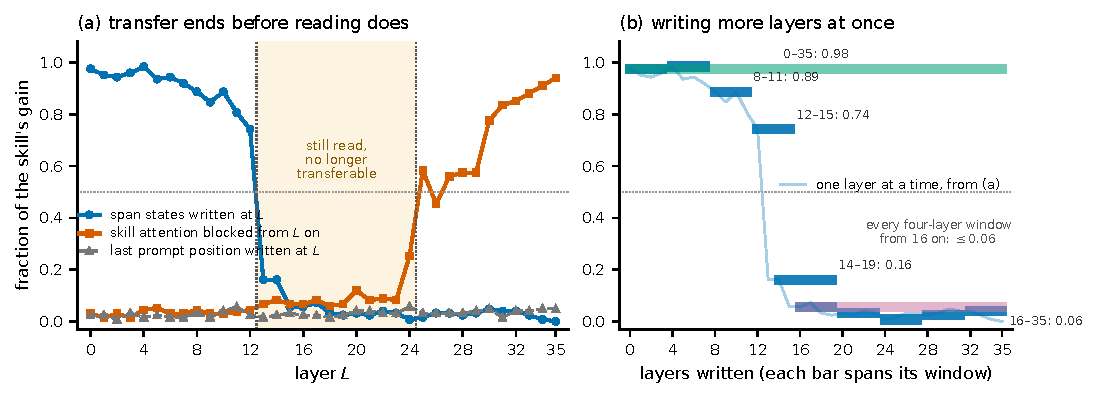
\includegraphics[width=0.96\textwidth]{fig-transfer-reading.pdf}
\caption{Transfer declines earlier than dependence on skill attention,
Qwen3-8B on MedCalc, with every layer measured. (a) Three interventions on
one axis and the same screened items ($n=135$; the knockout on their $134$
rescued items): span states written at layer $L$; attention to the skill
blocked from $L$ onward; and the last prompt position written at $L$. The
shaded band spans the layers where the skill is still read but no longer
transferable. (b) Each window is drawn across the layers it writes: four-layer
windows tile the stack, and the long windows $14$--$19$, $16$--$35$ and
$0$--$35$ are shown with them; the faint curve repeats (a). Writing every
layer at once recovers $0.98$, while any window starting at $16$ or later
stays at or below $0.06$. Span interventions use the corrected implementation;
attention knockout does not use state capture.}
\label{fig:transferreading}
\end{figure*}

\begin{table*}[tbp]
\caption{Replication with the corrected implementation. Injection layers are
$8$ for Qwen3-8B, $6$ for Qwen3-0.6B and $4$ for Mistral-7B. Recovery
intervals resample skill groups. Max control includes half-dose, other-skill,
permutation and noise comparisons, including same-family means available on
$41$ MedCalc/Qwen3-8B and $31$ MedCalc/Mistral items. $n$ describes the battery.
Handover brackets the transfer boundary as a fraction of model depth; reading
is the first layer, at one-layer resolution, from which blocking attention to
the skill still leaves at least half of the rescued items correct, measured on
the same screened items as the transfer boundary. $k^{*}$ is the rank knee on
the fixed grid.}
\label{tab:replication}
\centering
\footnotesize
\setlength{\tabcolsep}{4pt}
\begin{tabular}{@{}llrccccc@{}}
\toprule
task & model & $n$ (groups) & $\rho$ [95\% CI] & max control & handover & reading & $k^{*}$ \\
\midrule
MedCalc & Qwen3-8B & $135$ ($14$) & $0.89$ $[0.76,0.97]$ & $0.12$ & $0.33$--$0.36$ & $0.69$ & $47$ \\
TheoremQA & Qwen3-8B & $99$ ($75$) & $0.84$ $[0.75,0.92]$ & $0.25$ & $0.33$--$0.36$ & $0.58$ & $50$ \\
MedCalc & Qwen3-0.6B & $362$ ($38$) & $0.91$ $[0.75,1.05]$ & $0.30$ & $0.36$--$0.39$ & $0.79$ & $43$ \\
TheoremQA & Qwen3-0.6B & $132$ ($97$) & $0.74$ $[0.66,0.82]$ & $0.13$ & $0.36$--$0.39$ & $0.71$ & $52$ \\
MedCalc & Mistral-7B & $92$ ($20$) & $0.84$ $[0.69,1.09]$ & $0.35$ & $0.19$--$0.22$ & $0.84$ & $72$ \\
TheoremQA & Mistral-7B & $115$ ($94$) & $0.94$ $[0.84,1.05]$ & $0.27$ & $0.19$--$0.22$ & $0.59$ & $64$ \\
\bottomrule
\end{tabular}

\end{table*}

\paragraph{Adding late intervention layers does not restore transfer.}
To test whether a single late injection is simply too weak, we replace span
states repeatedly within consecutive layer windows, using the battery's
receiver and the same $135$ items as the depth sweep. Windows $8$--$11$,
$12$--$15$, $14$--$19$ and $16$--$35$ recover $0.89$, $0.74$, $0.16$ and
$0.06$; the last equals layer $16$ alone. Writing every layer at once
recovers $0.98$ [$0.91,1.03$], so the transplant itself remains effective when
it starts early enough; the identity control is exact on all $467$ items. On
TheoremQA ($99$ items, $75$ groups, with its battery's receiver), the same
windows recover $0.84,0.61,0.38,0.20$, the last again equal to layer $16$
alone. Repeated late injection therefore does not restore early-layer
recovery in these tests.

\paragraph{A spectral drop is not evidence of compression.}
Could the loss of transfer reflect compression into fewer dimensions? We
examine the centred participation ratio, a summary of how broadly matrix energy
is distributed across singular directions. It falls from $68$ at layer $12$
to $1.0$ at layer $16$, but this drop is driven by unusually large activations
\citep{sun2024massive, shi2026melayer}. In $35$ of $48$ calculators, one
token's state reaches $121$--$195$ times the median span norm, always on the
same two hidden dimensions. Removing the four highest-norm positions restores
the ratio to $85$ at layer $16$, and it stays between $62$ and $98$ over layers
$0$--$28$. The drop is also absent in Qwen3-0.6B and Qwen3-1.7B.
This diagnostic therefore does not support compression as the explanation
for lost transfer: a few large activations distort the dimensionality summary
(\extref{Appendix Table}{tab:prdiag}{extended version}).

\subsection{Replication across models and task domains}
\label{sec:ladder}

We extend span injection, rank truncation and the available depth comparisons
to Qwen3-0.6B ($D=1024$), Mistral-7B ($D=4096$, $32$ layers), and TheoremQA.
Each model is injected at an early layer, and the receiver screen is applied
separately to each run. Table~\ref{tab:replication} distinguishes completed
comparisons from missing controls or attention knockouts. Results for
Qwen3-1.7B, where skills rescue only $8$--$11\%$ of items, appear in \extref{Appendix Table}{tab:laddermodels}{the extended version}.

Span recovery ranges from $0.74$ to $0.94$ across the six model--task
combinations. The largest control is $0.35$, for a same-family
mean on $31$ Mistral/MedCalc items, where full-span recovery on the same items
is $0.71$. In every model--task combination, the transfer boundary occurs
before the reading boundary. The measured transfer boundaries lie at
$0.33$--$0.43$ of model depth within Qwen and at $0.19$--$0.22$ in Mistral.
Reading boundaries also vary by task: $0.58$--$0.71$ on TheoremQA and
$0.69$--$0.84$ on MedCalc across the three models.

The pre-registered width-proportional prediction places Qwen3-0.6B's rank
knee near $12$. Its observed recovery at $k=16,32,64,128$ is
$0.00,0.12,0.79,0.67$, giving $k^{*}=43$ [$39,52$], close to Qwen3-8B's
$47$ [$43,55$] despite the fourfold width difference. On TheoremQA, the
corresponding knees are $52$ [$46,62$] and $50$ [$39,67$], again inconsistent
with proportional scaling. Their participation ratios are also similar in
scale ($65$--$75$ versus $70$--$99$ over layers $0$--$20$, excluding unusually
large activations). Mistral, with the same width as Qwen3-8B, gives
$k^{*}=72$ [$46,94$] on MedCalc and $64$ [$50,79$] on TheoremQA: higher than
Qwen3-8B on both tasks, but with overlapping intervals. Its curve is also less
sharply defined, since recovery keeps rising past $k=128$ ($0.54$; $0.72$ at
$256$) and reaches its untruncated $0.84$ at $k=384$, against $256$ for
Qwen3-8B; its bottom-$k$ controls reach
$0.11$--$0.21$. The measured rank requirement is therefore not determined by
hidden width alone, while a difference between families is not established.

\paragraph{Readout checks.}
\label{sec:traps}
Alternative readouts can rank interventions differently. On the synthetic task,
averaged gold-answer log-probability favours a mean shared across skills by
$5.05$ nats despite lower accuracy ($0.251$ versus $0.288$, $358$ items).
Forcing an \texttt{ANSWER:} cue on MedCalc cuts the skill's accuracy gain from
$39.7$ to $4.7$ points ($0.178$ versus $0.131$ on $720$ items) while leaving a
$+1.08$ nat log-probability difference. Synthetic multiple
choice retains $0.54$ of the skill's effect after its numbers are corrupted and
$0.82$ after its lines are scrambled, illustrating possible answer-format
shortcuts
\citep{balepur2024artifacts} (\extref{Appendix}{app:traps}{extended version}). Other domains give limited evidence
(\extref{Appendix}{app:replication}{extended version}).

